\documentclass{standalone}
\usepackage{tikz}
\begin{document}
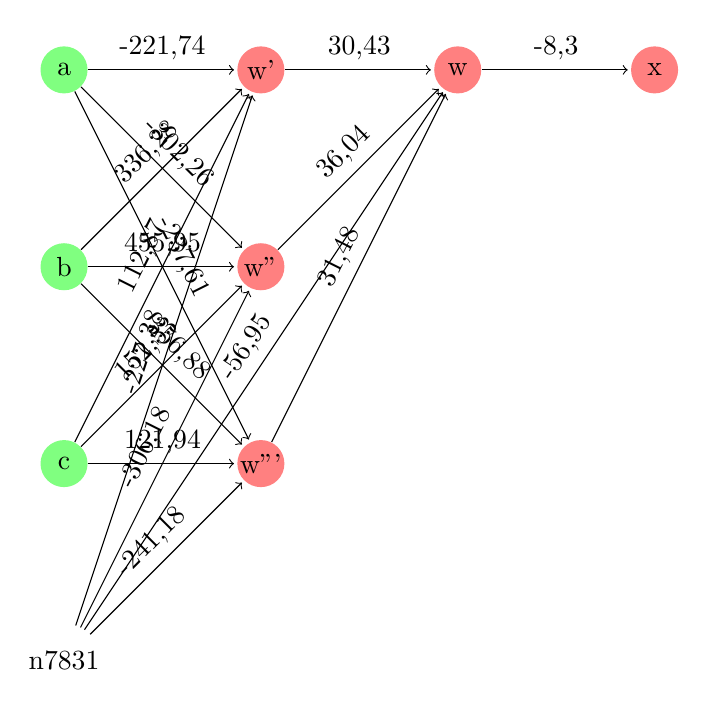
\begin{tikzpicture}[shorten >=1pt,->,draw=black!,node distance=2.5cm]
\tikzstyle{neuron}=[circle,fill=black!25,minimum size=17pt,inner sep=0pt]
\tikzstyle{constant}=[neuron, fill=white!50];
\tikzstyle{identity}=[neuron, fill=green!50];
\tikzstyle{sigmoid}=[neuron, fill=red!50];
\node [identity] (a) {a};
\node [identity,below of=a] (b) {b};
\node [identity,below of=b] (c) {c};
\node [constant,below of=c] (n7831) {n7831};
\node [sigmoid,right of=a] (w') {w'};
\node [sigmoid,below of=w'] (w'') {w''};
\node [sigmoid,below of=w''] (w''') {w'''};
\node [sigmoid,right of=w'] (w) {w};
\node [sigmoid,right of=w] (x) {x};
\path[every node/.style={sloped,anchor=south,auto=false}]
(a) edge node {-237,61} (w''')
(a) edge node {-221,74} (w')
(a) edge node {-302,26} (w'')
(c) edge node {112,87} (w')
(c) edge node {152,53} (w'')
(c) edge node {121,94} (w''')
(b) edge node {336,28} (w')
(b) edge node {455,95} (w'')
(b) edge node {356,88} (w''')
(w'') edge node {36,04} (w)
(w') edge node {30,43} (w)
(w) edge node {-8,3} (x)
(w''') edge node {31,48} (w)
(n7831) edge node {-227,38} (w')
(n7831) edge node {-56,95} (w)
(n7831) edge node {-241,18} (w''')
(n7831) edge node {-306,18} (w'')
;\end{tikzpicture}
\end{document}